Para hacer los experimentos, implementamos un generador de instancias pseudo-aleatorio. Recibe un valor $n$ como parámetro y genera
un sistema de $n$ nodos. Para todo $i,j$, (con la excepción de $i=j$), existe una probabilidad de 0.1 de que exista un link saliente
entre $i$ y $j$.

\subsection{Iteraciones de power method con y sin mejoras} 

\begin{figure}[!h]
        \begin{center}
                  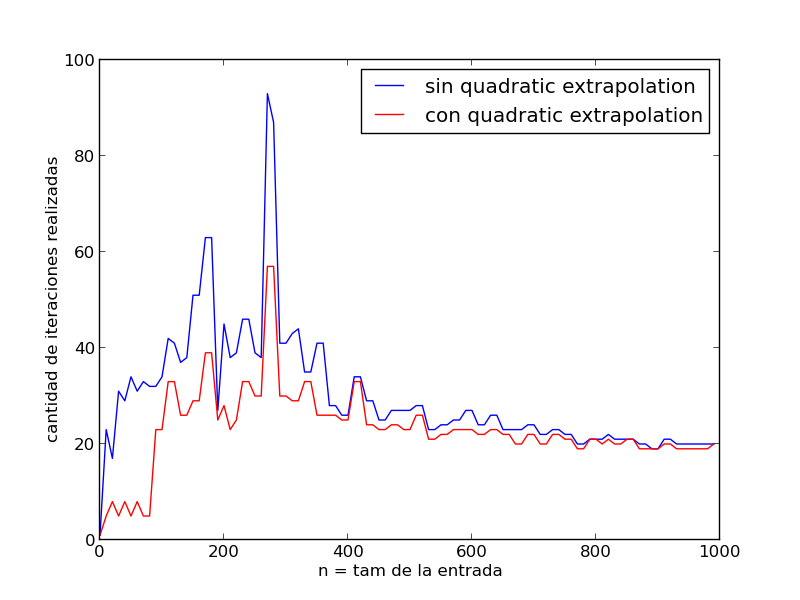
\includegraphics[scale = 0.6]{graficos/vs.png}
                  \caption{Iteraciones en función de cantidad de nodos}
                  \label{fig:contra1}
        \end{center}
\end{figure}
\FloatBarrier

El experimento fue realizado corriendo ambos algoritmos para 100 instancias de $i*10$ nodos,
con $0 \leq i \leq 99$.
Como podemos observar en la figura, la implementación que aplica Quadratic extrapolation realiza menos iteraciones
que la que no posee la optimización. Una particularidad que puede observarse consiste en que para valores mayores de $n$, la diferencia
la cantidad de iteraciones realizadas por ambos métodos disminuye.

\subsection{Experimento 2: Variando la periodicidad de Extrapolaci\'on cuadr\'atica}

Si bien el m\'etodo de extrapolaci\'on cuadr\'atica ayuda a la convergencia general del m\'etodo de la potencia, su costo es mucho mayor al ciclo principal del m\'etodo mencionado. Es por esto que, para realmente acelerar el ritmo de convergencia es necesario realizar la extrapolaci\'on cuadr\'atica de manera peri\'odica y no en cada iteraci\'on.

Pero, ¿Cual es la distancia \'optima entre iteraciones en las que debemos realizar la extrapolaci\'on? ¿Disminuyen las iteraciones totales si se aplica la extrapolaci\'on cuadr\'atica de manera cercana? ¿Y qu\'e sucede con el tiempo?

Para responder a todas estas preguntas, planteamos dos pequeños experimentos en base al grafo $web-Stanford$ de aproximadamente 280mil nodos:

\begin{itemize}
	\item Analizar la relaci\'on periodicidad-\#IteracionesTotales variando la distancia entre iteraciones en las que usamos la Extrapolaci\'on Cuadr\'atica.
	\item Analizar la relaci\'on periodicidad-tiempo operando de la misma forma que en el item anterior pero realizando varias repeticiones de cada experimento para promediar los tiempos y evitar valores incoherentes propios del scheduling de nuestro sistema operativo.
\end{itemize}

~

Los resultados fueron los siguientes:

\begin{center}
    \small{
    \begin{tabular}{| l | l |}
    \hline
    Distancia entre iteraciones con extrapolaci\'on & \#Iteraciones\_Totales \\ \hline
    5 & 75 \\ \hline
    7 & 71 \\ \hline
    10 & 71 \\ \hline
    20 & 73 \\ \hline
    30 & 72 \\ \hline
    40 & 74 \\ \hline
    50 & 74 \\ \hline

    \end{tabular}
    }
\end{center}
\begin{center}
c = 0.80. Epsilon = $10^{-10}$.
\end{center}

~

Si bien la cantidad de iteraciones totales disminuye con extrapolac\'ion cuadr\'atica respecto del m\'etodo cl\'asico de la potencia, puede apreciarse en la tabla que su periodicidad en la aplicaci\'on no modifica en gran medida la cantidad total de iteraciones para el mismo m\'etodo, contrario a lo que cre\'iamos inicialmente. 

Sin embargo, fue notorio durante el trayecto de este experimento que los tiempos iban cambiando a medida que se produc\'ian menos llamadas a extrapolaci\'on cuadr\'atica, lo cual era de esperarse debido al costo dicho m\'etodo.

Seg\'un estos resultados, creemos que realizar extrapolaci\'on cada 10 iteraciones es un buen criterio para minimizar la cantidad de ciclos en base a un grafo de entrada de caracter\'isticas similiares.

~

A continuaci\'on, los resultados obtenidos respecto del tiempo total de ejecuci\'on. 


\begin{center}
    \small{
    \begin{tabular}{| l | l |}
    \hline
    Distancia entre iteraciones con extrapolaci\'on & Tiempo (en millones de ciclos) \\ \hline
    7 & \textcolor{red}{\~21} \\ \hline
    10 & 16.4
    15 & 12.06 \\ \hline
    25 & 9 \\ \hline
    35 & 8.85 \\ \hline
    45 & 7.48 \\ \hline
    
    \end{tabular}
    }
\end{center}
\begin{center}
c = 0.80. Epsilon = $10^{-10}$. Tiempos medidos en base a $tiempo.h$ otorgado por la c\'atedra de Orga2.
\end{center}

Dado que el algoritmo de power-method-with-quadratic-extrapolation es costoso en terminos de tiempo con grafos de entrada suficientemente grandes, se realizaron s\'olo 5 repeticiones de las mediciones para acortar tiempos. 

Podemos apreciar el gran costo de aplicar el m\'etodo de extrapolaci\'on cuadr\'atica de forma $demasiado$ peri\'odica viendo el tiempo total que tarda el algoritmo si las iteraciones de extrapolaci\'on son muy cercanas.

Observando la tabla podemos ver que el tiempo disminuye a medida que se aplica el m\'etodo de manera mas distanciada, acelerando la convergencia de manera periodica sin retrasar el tiempo total con sucesivas llamadas al costoso proceso de extrapolaci\'on cuadr\'atica.







\subsection{Variando el valor de c}

Antes de realizar cualquier experimentación nos pareció que un valor de $c=0.8$ era muy razonable, ya que respeta las condiciones
originales del problema. El navegante de la web normalmente sigue los links de las páginas, y en alguna que otra ocasión decide
introducir una nueva url.

Al disminuír el valor de $c$, y por lo tanto aumentar el de $(1-c)$, lo que estamos haciendo en realidad es homogeneizar los valores
del vector estacionario final, ya que aumentan las probabilidades de realizar saltos aleatorios. Cuando esto sucede, disminuye
la probabilidad de que un navegante de la web permanezca en una única pág.

Por el contrario, cuando $c=1$ se respeta por completo la instancia inicial, y la diferencia entre el máximo y el mínimo módulo
de los elementos del vector estacionario va a ser menor.

\begin{figure}[!h]
        \begin{center}
                  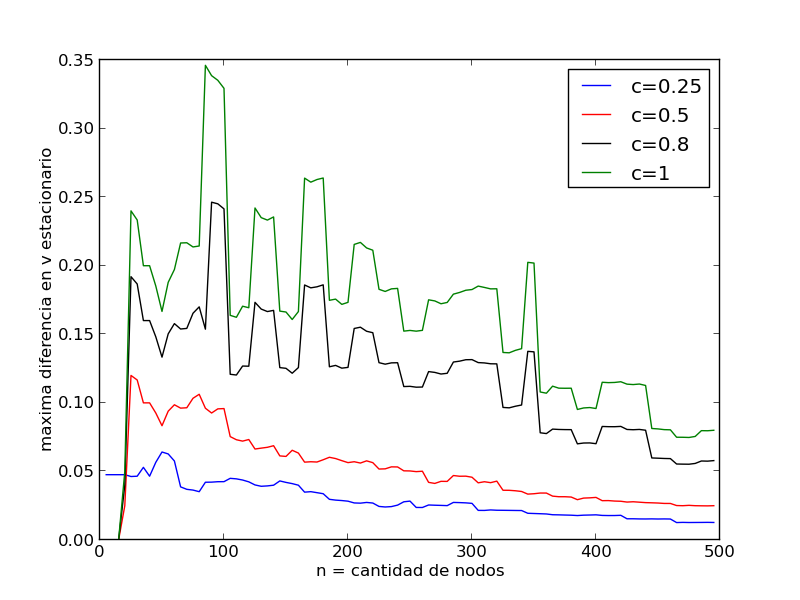
\includegraphics[scale = 0.6]{graficos/variando_c.png}
                  \caption{Variacion entre max y min módulo para distintos valores de c}
                  \label{fig:contra1}
        \end{center}
\end{figure}
\FloatBarrier

